\section{Systemfunktionen}
Wir haben die Systemfunktionen nach Usergruppen aufgeteilt. 

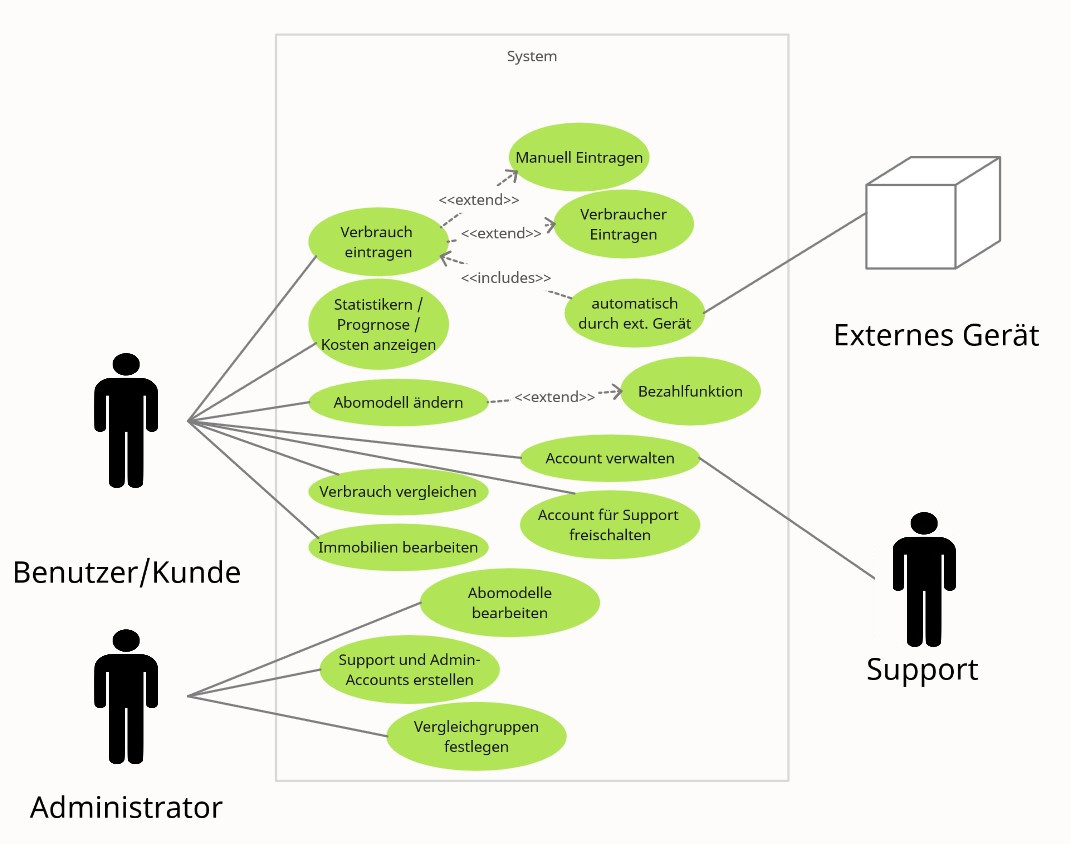
\includegraphics[scale=0.5]{UC.jpg}

\subsection{Systemfunktionen für alle Usergruppen}
\subsubsection{Anmeldung}
\paragraph{Beschreibung und Priorität}
\paragraph{Sequenzen von Benutzeraktionen und Systemantworten}
\paragraph{Funktionale Anforderungen}

\subsection{Benutzer}
\subsubsection{Accounterstellung}\label{acc}
\paragraph{Beschreibung und Priorität}
Diese Funktion ermöglicht es, einer Person, die an dem Produkt interessiert ist, ein Account anzulegen und somit anfangen kann das Produkt zu nutzen. Die Priorität dieser Funktion kann nicht überschätzt werden, da ohne sie, keine der Folgenden umsetzbar wäre.
\paragraph{Sequenzen von Benutzeraktionen und Systemantworten} Der/die Interessierte gibt in der Anmelde-Maske ihren frei gewählten Benutzername, ihre E-Mail-Adresse und schließlich ein Passwort ein. Nach einem Knopfdruck, wird, wenn die Eingaben die funktionalen Anforderungen REG4, REG5, REG6 erfüllen, der Benutzer nun auf die Startseite weitergeleitet. Wenn nicht, wird der Benutzer über die nicht erfüllten Anforderungen in der Anmelde-Maske informiert und kann daraufhin seine/ihre Eingaben anpassen.
\paragraph{Funktionale Anforderungen}
\begin{itemize}
	\item \textbf{REG1} Darstellen der Anmelde-Maske
	\item \textbf{REG2} Validieren den Eingabe also Überprüfung von REG4, REG5, REG6  durch ggf. Abgleich mit der Datenbank
	\item \textbf{REG3} Auf nicht erfüllte Anforderungen (REG4, REG5, REG6) in der Anmeldemaske aufmerksam machen, falls diese nicht erfüllt sind.
	\item \textbf{REG4} Kein 2 Benutzer dürfen den selben Benutzername haben.
	\item \textbf{REG5} Das Passwort muss dem folgenden Standard genügen:
	\begin{itemize}
		\item Mindestlänge: 8 Zeichen
		\item Enthält min. einen deutschen Großbuchstaben (A-Z, Ä, Ö, Ü)
		\item Enthält min. einen deutschen Kleinbuchstaben (a-z, ä, ö, ü, ß)
		\item Enthält min. eine arabische Ziffer (0-9)
		\item Enthält min. ein Zeichen, dass nicht in die bisherigen Kategorien passt (!, \$, \#, \%, ...)
	\end{itemize}
	\item \textbf{REG6} Die eingegebene E-Mail-Adresse muss im richtigen Format sein.
	
\end{itemize}

\subsubsection{Verbräuche eintragen}
\paragraph{Beschreibung und Priorität}
Es ermöglicht dem Benutzer seine Daten in die Datenbank einzutragen, welche später für weitere Features von nöten sind. Neben dem manuellen Eintragen gibt es auch die Möglichkeit der automatischen Erfassung der Daten mittels einem Gerät, das der Benutzer zuhause installieren muss, sobald dies passiert ist übermittelt das Gerät jeden Tag die aktuellen Daten… oder so.

\paragraph{Sequenzen von Benutzeraktionen und Systemantworten}
Der Benutzer trägt in einer WebMaske seine einzelnen Verbräuche ein und kann mit einem Klick auf den Button “hochladen” seine Daten der Datenbank hinzufügen, bevor dies geschieht, wird aber überprüft, ob die Daten neu und sinnig sind.
\paragraph{Funktionale Anforderungen}

\subsubsection{Statistiken einsehen}
\paragraph{Beschreibung und Priorität}
\paragraph{Sequenzen von Benutzeraktionen und Systemantworten}
\paragraph{Funktionale Anforderungen}

\subsubsection{Immobilien bearbeiten}
\paragraph{Beschreibung und Priorität}
Der Benutzer kann Immobilien hinzufügen,
bearbeiten und entfernen. %was soll das noch können?
% Ein Benutzer sollte(?) für das Eintragen von Wasser-/Gas-/ Stromverbrauch 
% mindestens eine Immobilie angeben mit Informationen über den Flächeninhalt 
% und Anzahl der Haushaltsmitglieder für eine möglichst genaue Analyse über den Verbrauch des Nutzers verglichen mit dem Durchschnitt. 
Diese Funktion hat keine hohe Priorität(?) da sie nur für den Vergleich mit dem Durchschnitt relevant ist. 
\paragraph{Sequenzen von Benutzeraktionen und Systemantworten}
Der Benutzer wählt in seinem Profil aus, 
dass er seine Immobilien bearbeiten möchte. 
Dabei bekommt er die Option, eine neue Immobilie anzulegen, 
oder von vorhandenen Immobilien eine zu bearbeiten. 
Wenn er das erste aussucht, kann man eine Bezeichnung,
Flächeninhalt und Haushaltsgröße % noch was?
eintragen. Die Bezeichnung ist zwingend notwendig, %(?)
die anderen Angaben nicht. 
Der Nutzer kann sich dazu entscheiden, den Vorgang abzubrechen.
Wenn der Nutzer eine vorhandene Immobilie bearbeiten will,
dann werden ihm ebenfalls angeboten, Bezeichnung, Flächeninhalt und 
Haushaltsgröße zu ändern,
zusätzlich hat er die Option, die ganze Immobilie zu löschen. 
Wenn der Nutzer etwas bearbeitet hat, bekommt er die Option, seine Änderungen zu speichern. 
Wenn er das auswählt, dann ist der Bearbeitungsvorgang abgeschlossen.

Wenn der Nutzer sich für das Löschen entscheidet, wird er final gewarnt, 
dass das Löschen einer Immobilie alle damit verbundenen Daten löscht und der Vorgang nicht widerrufbar ist.  
%klingt momentan sehr dumm muss geändert werden
Wenn der Nutzer zugestimmt hat, dass ihm das bewusst ist und trotzdem fortfahren will, dann wird die Immobilie und alle Daten die damit verbunden waren aus der Datenbank entfernt.

\paragraph{Funktionale Anforderungen}

% Müssen wir dazu schreiben, was das Character Limit ist? 
%dass Flächen  und Haushaltsgröße nur mit Zahlen angegeben werden können? 
%Was wir mit ungültigen Antworten machen?
\begin{itemize}
    \item Wenn noch keine Immobilie angelegt wurde, gibts auch keine Option, etwas bearbeiten zu können (?)
    \item Die Bezeichnung kann alle möglichen ASCII-Zeichen (?) beinhalten.
    \item Der Flächeninhalt kann nur in positiven Fließkommazahlen/ ganzen Zahlen angegeben werden.
    \item Die Haushaltsgröße kann nur in positiven ganzen Zahlen angegeben werden
    \item ???
\end{itemize}

\subsubsection{Abomodell ändern}
TODO: Text an Pfeile

\begin{tikzpicture}[object/.style = {draw, rectangle}, activity/.style = {draw, rounded corners=0.1cm}, split/.style = {draw, diamond}] 
	\node[circle, fill] (start) {};
	\node[object] (1) [below of=start] {Abomodell ändern};
	\node[activity] (2) [right of=1, node distance=4cm] {Modell wählen};
	\node[activity] (3) [right of=2, node distance=4cm] {Startzeitpunkt wählen};
	\node[split] (s1) [below of=1] {};
	\node[split] (s2) [below of=s1] {};
	\node[activity] (4) [right of=s2, node distance=5cm] {Modell auf \textit{Frei} setzen};
	\node[circle, fill] (unabo) [right of=4, , node distance=3cm] {};
	\node[split] (s3) [below of=s2] {};
	\node[activity] (5) [right of=s3, node distance=5cm] {Rechnungsadresse eintragen};
	\node[split] (s4) [below of=s3] {};
	\node[activity] (6) [below of=s4] {Bezahlungmethode wählen};
	\node[activity] (7) [right of=6,  node distance=5cm] {Bezahlung durchführen};
	\node[split] (s5) [right of=7,  node distance=3.5cm] {};
	\node[object] (8) [below of=s5] {Bestätigung};
	\node[activity] (9) [right of=s4, node distance=6.7cm] {Abbrechen};
	\node[circle, fill] [right of=9, node distance=1.35cm] (cancel) {};
	\node[activity] (10) [left of=8, node distance=3cm] {Abomodell setzen};
	\node[circle, fill] [left of=10, node distance=2cm] (finish) {};
	
	
	\draw[->] (start) -- (1);
	\draw[->] (1) -- (2);
	\draw[->] (2) -- (3);
	\draw[->] (3) -- (s1);
	\draw[->] (s1) to [out=0,in=270, looseness=0.3] (3);
	\draw[->] (s1) -- (s2);
	\draw[->] (s2) -- (4);
	\draw[->] (4) -- (unabo);
	\draw[->] (s2) -- (s3);
	\draw[->] (s3) -- (5);
	\draw[->] (s3) -- (s4);
	\draw[->] (5) -- (s4);
	\draw[->] (s4) -- (6);
	\draw[->] (6) -- (7);
	\draw[->] (7) -- (s5);
	\draw[->] (s5) -- (8);
	\draw[->] (s5) to [out=90,in=0,looseness=0.1] (s4);
	\draw[->] (s4) --(9);
	\draw[->] (9) --(cancel);
	\draw[->] (8) --(10);
	\draw[->] (10) -- (finish);
\end{tikzpicture}
\paragraph{Beschreibung und Priorität}
Der Benutzer kann hiermit zwischen Abomodellen wechseln. Geplant sind die Abomodelle \textit{Frei}, \textit{Standart} und \textit{Professionell} wovon Ersteres kostenlos und standardmäßig ausgewählt sein sollte. Diese Funktion enthält neben dem Auswählen des Modells die Zahlung und Überprüfung vertraglicher Kündigungsfristen. Die Funktion gehört nicht zu den Kernanforderungen jedoch kann ohne Sie kein Umsatz erzielt werden und hat daher trotzdem eine hohe Priorität. 
\paragraph{Sequenzen von Benutzeraktionen und Systemantworten}
Nach der Auswahl des gewünschten Abomodells, muss, falls sich der User für ein kostenpflichtiges Modell entscheidet, man einen Startzeitpunkt (nach Richtlinie ABO3) entscheiden. Nach der Eingabe von Rechnungsadresse, die, falls Sie für den Benutzer schon bekannt ist, auch schon vor eingetragen sein sollte, kann der Benutzer eine präferierte Zahlungsmethode anwählen, wodurch er/sie zu einem externen Zahlungsdienstleister weitergeleitet wird. Schließlich kann der Prozess abgeschlossen werden und das neue Abomodell wird zum angegebenen Startzeitpunkt gesetzt. Eine Bezahlbestätigung wird versendet. Der Vorgang kann zu jedem Zeitpunkt abgebrochen werden.

\paragraph{Funktionale Anforderungen}
\begin{itemize}
	\item \textbf{ABO1} Darstellen der Maske zum Auswählen des Abomodells und Eintragen von Startzeitpunkt und Rechnungsdresse.
	\item \textbf{ABO2} Validieren der Eingabe des Startzeitpunkts (nach ABO3) und Reflektieren möglicher Fehler in der Maske
	\item \textbf{ABO3} Der Startzeitpunkt muss folgenden Richtlinien genügen:
	\begin{itemize}
		\item Er muss in der Zukunft liegen oder am derzeitigen Tag sein
		\item Falls die Kündigungszeitraum eines laufendes Abos noch nicht abgelaufen ist, muss der Startzeitpunkt nach Ablauf dieses Zeitraums liegen
	\end{itemize}
	\item \textbf{ABO4} Grundlegende Format-Überprüfungen der Rechnungsadresse (zB Postleitzahl besteht aus Zahlen etc.) und sollen bei Nichteinhaltung in der Maske kommuniziert werden
	\item \textbf{ABO5} Eine Verbindung zu sämtliche externen Zahlungsanbietern muss aufgebaut werden. Derzeit sind \textit{PayPal}, per Lastschrift, Sofort-Überweisung der \textit{Sofort GmbH}, \textit{Klarna}, mit Kreditkarte ???
	\item \textbf{ABO6} Schaffen einer Möglichkeit in jedem Schritt den Prozess abzubrechen
	\item \textbf{ABO7} Versenden einer Bezahlbestätigung
	\item \textbf{ABO8} Setzen des neuen Abomodells in den Benutzerdaten zum angegebenen Startzeitpunkt
\end{itemize}

\subsubsection{Account für Support freischalten}
\label{sys_feat:freischalten}
\paragraph{Beschreibung und Priorität}
Diese Funktion ermöglicht es dem Benutzer bei Problemen seinen Account für den Support freizuschalten, sodass der Support Änderungen vornehmen kann und gleichzeitig wird so die DSGVO eingehalten, was sehr wichtig für das System ist.
\paragraph{Sequenzen von Benutzeraktionen und Systemantworten} 
Der Benutzer hat mit der Nutzung des Systems ein Problem und benötigt Hilfe. Nachdem er das FAQ zur Handhabung des Systems gelesen hat und er dort keine Lösung für sein Problem finden konnte, nutzt er die Supportfunktion, wo er mit einem Mitarbeiter in Kontakt kommt. Zuerst versucht der Support dem Nutzer ohne weitere Daten weiterzuhelfen, sollte dies das Problem immer noch nicht lösen, muss der Nutzer seinen Account für den Support freischalten. Dem Nutzer wird ein Code generiert, den er dem Support durch gibt und den der Support benötigt, um sich berechtigten Zugang zum Nutzeraccount zu verschaffen. Nun kann der  Support dem Nutzer optimal weiterhelfen, indem er Zugriff auf seinen Account hat.
\paragraph{Funktionale Anforderungen}
\begin{itemize}
	\item \textbf{REG1} Laufende Internet- und/oder Telefonverbindung.
	\item \textbf{REG2} Der generierte Code für den Nutzer besteht aus Zahlen und Buchstaben.
	\item \textbf{REG3} Der generierte Code von Nutzer muss unbedingt mit dem benötigten Code des Supports übereinstimmen.
	
\end{itemize}

\subsubsection{Account verwalten}

\subsubsection{Prognosen einsehen}

\subsubsection{Kosten einsehen}
\paragraph{Beschreibung und Priorität}
Die Funktion Kosten einsehen ermöglicht dem Nutzer die Kosten zu seinen Verbäuchen einzusehen. Vorausgesetzt ist hierbei dass der Nutzer entweder seine Strom- /Gas- /Wasserverträge zu Verfügung stellt, oder die Kosten manuell einträgt. Sofern der Nutzer dies getan hat, kann er sich die Kosten für seine Verbräuche ansehen. Zudem kann er sich bei eigenen Verbrauchstypen auch eigene Kosten eintragen. Beispiel: Der Nutzer hat den Verbrauchstyp Anzahl an Kaffee pro Tag. Dazu kann der Nutzer nun einen Preis eintragen: Ein Kaffee kostet einen Euro. 
\paragraph{Sequenzen von Benutzeraktionen und Systemantworten}
Der Nutzer muss einen Verbrauchstyp auswählen und dann zu diesem Typ einen Zeitraum wählen. Danach werden ihm die Kosten für den Verbrauch über den Zeitraum angezeigt. Wenn der Nutzer seinen Verbrauch vergleicht, ist neben dem Vergleich des Verbrauchs auch ein Vergleich der Kosten sichtbar. 

\subsubsection{Verbrauch vergleichen}


\subsection{Support}
\subsubsection{Account eines Users verwalten}
\paragraph{Beschreibung und Priorität}
Ein Support-Benutzer muss in der Lage sein etwaige Benutzerdaten auf Anfrage des jeweiligen Benutzers zu ändern. Dafür muss allerdings das Einsehen der Benutzerdaten für den Supportbenutzer freigschaltet werden (siehe \ref{sys_feat:freischalten}). Diese Funktion ist nicht teil der Kernanforderungen, jedoch muss es unbedingt Teil der ersten Version sein, da die Kundenzufriedenheit davon abhängig ist. Daher ergibt sich eine mittlere Priorität.
\paragraph{Sequenzen von Benutzeraktionen und Systemantworten}
Der Support-Benutzer kann den Benutzer auswählen, dessen Stammdaten bearbeitet werden soll. Dabei werden dem Support-Benutzer nur diejenige Benutzernamen angezeigt, die die Barbeitung freigeschaltet hasben. Danach wird eine Oberfläche angezeigt, die der Oberfläche vom Bearbeiten der eigenen Stzammdatan eines Benutzers ähnelt. Hier können nun die Änderungen vorgenommen und gespeichert werden. 
\paragraph{Funktionale Anforderungen}
\begin{itemize}
	\item \textbf{SMG1} Zeige alle Benutzer, die die Bearbeitung nach \ref{sys_feat:freischalten} freigeschaltet haben.
	\item \textbf{SMG2} Bearbeiten aller Stammdaten eines Benutzers in der Oberfläche ermöglichen.
	\item \textbf{SMG3} Speichern der veränderten Daten. 
\end{itemize}

\subsection{Admin}
\subsubsection{Abomodelle modifizieren}
\paragraph{Beschreibung und Priorität}
Der Admin kann hiermit alle drei verfügbaren Abomodelle (Frei, Standard und Professionell) grundlegend ändern. Alle Abomodelle haben verschiedene Funktionen, welche der Admin anpassen kann. Der Admin hat die Möglichkeit die Kosten der verschieden Modelle anzupassen, Funktionen freischalten und Funktionen einschränken oder sogar ganz entfernen. Falls der Admin die Kosten eines Modells ändert, oder Funktionen hinzufügt oder entfernt, müssen gesetzliche Regelungen für Vertragsänderungen eingehalten werden. Das heißt Nutzer dieses Abomodells müssen benachrichtigt werden und es muss Ihnen eine Möglichkeit gegeben werden, das Abomodell zu kündigen. Das passiert unabhängig davon, ob der Admin die Kosten erhöht oder verringert, oder Funktionen hinzufügt oder entfernt. 
\paragraph{Sequenzen von Adminaktionen und Systemantworten}
Falls der Admin Abomodelle modifizieren will, muss der Admin gemäß ABOM3 einen Startzeitpunkt wählen, ab dem die Änderungen gültig werden. Dem Admin soll bekannt gemacht werden, ob der Zeitpunkt zu Nahe gewählt ist. Danach kann der Admin aus folgenden Funktionen wählen:
\begin{itemize}
	\item Vorhanden Funktion bearbeiten oder entfernen (Funktion muss in dem Abomodell momentan verfügbar sein).
	\item Eine neue Funktion hinzufügen
	\item Den Preis des Abomodells ändern
\end{itemize}
Wenn der Admin sich für eine der Funktionen entschieden hat, kann er diese ausführen und bestätigen sofern alles den Anforderungen entspricht. Der gesamte Vorgang kann jederzeit auch abgebrochen werden. Fährt der Admin fort, speichert das System die Änderungen und wendet diese zu dem gegebenen Zeitpunkt an.

\paragraph{Funktionale Anforderungen}
\begin{itemize}
	\item \textbf{ABOM1} Darstellen der Maske zum Auswählen des Abomodells und Eintragen von Startzeitpunkt.
	\item \textbf{ABOM2} Funktion entsprechend dem gewählten Abomodell muss änderbar und löschbar sein
	\item \textbf{ABOM3} Funktion soll hinzufügbar sein.
	\item \textbf{ABOM4} Ein neuer Preis für das Abomodell soll wählbar sein.
	\item \textbf{ABOM5} Der Startzeitpunkt muss in der Zukunft liegen und muss den gesetzlichen Regelungen entsprechen
	\item \textbf{ABOM6} Validieren der Eingabe des Startzeitpunkts (nach ABO5) und Reflektieren möglicher Fehler in der Maske
\end{itemize}


\subsubsection{Supportaccount erstellen???}

\subsubsection{Vergleichsgruppen festlegen???}
